% Construction : axe des rangs de 0 à 8, limite commune ℓ = 1.5.
%   v_n monte vers ℓ  : 0.5, 0.85, 1.1, 1.25, 1.34, 1.4, 1.44, 1.47
%   w_n descend vers ℓ : 2.5, 2.15, 1.9, 1.75, 1.66, 1.6, 1.56, 1.53
%   u_n reste entre les deux, sans monotonie :
%                        1.15, 1.95, 1.2, 1.7, 1.4, 1.55, 1.47, 1.51
%   Chaque famille est reliée par une ligne brisée, et nommée à gauche, là où
%   les trois sont encore écartées.
% SVG : x = 30 + 32x, y = 130 - 40y.
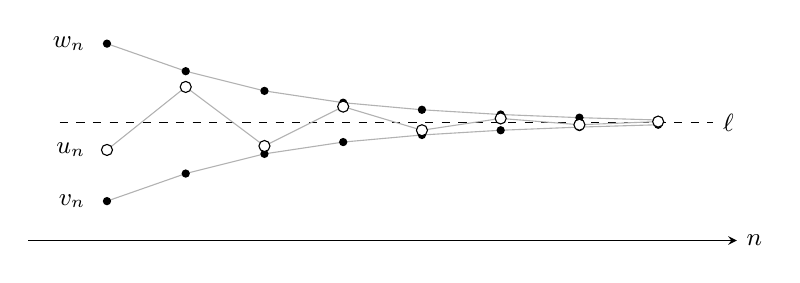
\begin{tikzpicture}[scale=1, >=stealth, every node/.style={font=\small}]
  \draw[->] (0, 0) -- (9, 0) node[right] {$n$};
  \draw[dashed] (0.4, 1.5) -- (8.7, 1.5) node[right] {$\ell$};
  \draw[gray!60] plot coordinates
    {(1,0.5) (2,0.85) (3,1.1) (4,1.25) (5,1.34) (6,1.4) (7,1.44) (8,1.47)};
  \draw[gray!60] plot coordinates
    {(1,2.5) (2,2.15) (3,1.9) (4,1.75) (5,1.66) (6,1.6) (7,1.56) (8,1.53)};
  \draw[gray!60] plot coordinates
    {(1,1.15) (2,1.95) (3,1.2) (4,1.7) (5,1.4) (6,1.55) (7,1.47) (8,1.51)};
  \foreach \n/\v in {1/0.5, 2/0.85, 3/1.1, 4/1.25, 5/1.34, 6/1.4, 7/1.44, 8/1.47}
    \fill (\n, \v) circle (1.5pt);
  \foreach \n/\v in {1/2.5, 2/2.15, 3/1.9, 4/1.75, 5/1.66, 6/1.6, 7/1.56, 8/1.53}
    \fill (\n, \v) circle (1.5pt);
  \foreach \n/\v in {1/1.15, 2/1.95, 3/1.2, 4/1.7, 5/1.4, 6/1.55, 7/1.47, 8/1.51}
    \draw[fill=white] (\n, \v) circle (2pt);
  \node[left] at (0.85, 2.5) {$w_n$};
  \node[left] at (0.85, 1.15) {$u_n$};
  \node[left] at (0.85, 0.5) {$v_n$};
\end{tikzpicture}
